\section{Introduction}
\label{sec:introduction}

A memory unit is a device to which binary information is transferred for storage and from which information is retrieved when needed for processing. When data processing takes place, information from memory is transferred to selected registers in the processing unit. A \textit{memory unit} is a \textit{collection of cells capable of storing a large quantity of binary information}.

There are two types of memories that are used in digital systems: 
\begin{itemize}
  \item random-access memory (RAM)
  \item read-only memory (ROM)
\end{itemize}
\noindent RAM stores new information for later use. The process of storing new information into memory is referred to as a memory \textit{write} operation. The process of transferring the stored information out of memory is referred to as a memory \textit{read} operation.

RAM can perform \textit{both write and read} operations. ROM can \textit{perform only the read} operation. This means that suitable binary information is already stored inside memory and can be retrieved or read at any time. However, that information cannot be altered by writing.

ROM is a \textit{programmable logic device} (\textbf{PLD}). The binary information that is stored within such a device is specified in some fashion and then embedded within the hardware in a process referred to as programming the device. The word ``programming'' here refers to a hardware procedure, which specifies the bits that are inserted into the hardware configuration of the device.

Figure 1 shows the conventional and array logic symbols for a multiple input OR gate.
\begin{figure}[H]
  \centering
  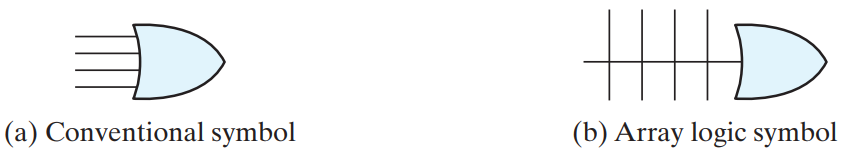
\includegraphics[width=\linewidth]{img/fig-7.1.png}
  \caption{Conventional and array logic diagrams for OR gate}
  \label{fig:7.1}
\end{figure}
